\documentclass[12pt,a4paper,]{report}
\usepackage{lmodern}
\usepackage{setspace}
\setstretch{1.5}
\usepackage{amssymb,amsmath}
\usepackage{ifxetex,ifluatex}
\usepackage{fixltx2e} % provides \textsubscript
\ifnum 0\ifxetex 1\fi\ifluatex 1\fi=0 % if pdftex
  \usepackage[T1]{fontenc}
  \usepackage[utf8]{inputenc}
\else % if luatex or xelatex
  \ifxetex
    \usepackage{mathspec}
  \else
    \usepackage{fontspec}
  \fi
  \defaultfontfeatures{Ligatures=TeX,Scale=MatchLowercase}
    \setmainfont[]{Calibri}
\fi
% use upquote if available, for straight quotes in verbatim environments
\IfFileExists{upquote.sty}{\usepackage{upquote}}{}
% use microtype if available
\IfFileExists{microtype.sty}{%
\usepackage{microtype}
\UseMicrotypeSet[protrusion]{basicmath} % disable protrusion for tt fonts
}{}
\usepackage[left=4cm,right=2.5cm,top=2.5cm,bottom=2.5cm]{geometry}
\usepackage{hyperref}
\hypersetup{unicode=true,
            pdftitle={Thesis},
            pdfauthor={Rebecca Anne Senior},
            pdfborder={0 0 0},
            breaklinks=true}
\urlstyle{same}  % don't use monospace font for urls
\usepackage{natbib}
\bibliographystyle{apalike}
\usepackage{longtable,booktabs}
\usepackage{graphicx,grffile}
\makeatletter
\def\maxwidth{\ifdim\Gin@nat@width>\linewidth\linewidth\else\Gin@nat@width\fi}
\def\maxheight{\ifdim\Gin@nat@height>\textheight\textheight\else\Gin@nat@height\fi}
\makeatother
% Scale images if necessary, so that they will not overflow the page
% margins by default, and it is still possible to overwrite the defaults
% using explicit options in \includegraphics[width, height, ...]{}
\setkeys{Gin}{width=\maxwidth,height=\maxheight,keepaspectratio}
\IfFileExists{parskip.sty}{%
\usepackage{parskip}
}{% else
\setlength{\parindent}{0pt}
\setlength{\parskip}{6pt plus 2pt minus 1pt}
}
\setlength{\emergencystretch}{3em}  % prevent overfull lines
\providecommand{\tightlist}{%
  \setlength{\itemsep}{0pt}\setlength{\parskip}{0pt}}
\setcounter{secnumdepth}{5}
% Redefines (sub)paragraphs to behave more like sections
\ifx\paragraph\undefined\else
\let\oldparagraph\paragraph
\renewcommand{\paragraph}[1]{\oldparagraph{#1}\mbox{}}
\fi
\ifx\subparagraph\undefined\else
\let\oldsubparagraph\subparagraph
\renewcommand{\subparagraph}[1]{\oldsubparagraph{#1}\mbox{}}
\fi

%%% Use protect on footnotes to avoid problems with footnotes in titles
\let\rmarkdownfootnote\footnote%
\def\footnote{\protect\rmarkdownfootnote}

%%% Change title format to be more compact
\usepackage{titling}

% Create subtitle command for use in maketitle
\newcommand{\subtitle}[1]{
  \posttitle{
    \begin{center}\large#1\end{center}
    }
}

\setlength{\droptitle}{-2em}
  \title{Thesis}
  \pretitle{\vspace{\droptitle}\centering\huge}
  \posttitle{\par}
  \author{Rebecca Anne Senior}
  \preauthor{\centering\large\emph}
  \postauthor{\par}
  \date{}
  \predate{}\postdate{}

\usepackage{booktabs}
\usepackage[table]{xcolor}
\definecolor{lightgrey}{gray}{0.85}
\usepackage{pdfpages}
\usepackage{rotating}
\usepackage{multirow}
\usepackage{array}
\usepackage{setspace}
\onehalfspacing

\usepackage{amsthm}
\newtheorem{theorem}{Theorem}[chapter]
\newtheorem{lemma}{Lemma}[chapter]
\theoremstyle{definition}
\newtheorem{definition}{Definition}[chapter]
\newtheorem{corollary}{Corollary}[chapter]
\newtheorem{proposition}{Proposition}[chapter]
\theoremstyle{definition}
\newtheorem{example}{Example}[chapter]
\theoremstyle{definition}
\newtheorem{exercise}{Exercise}[chapter]
\theoremstyle{remark}
\newtheorem*{remark}{Remark}
\newtheorem*{solution}{Solution}
\begin{document}
\maketitle

{
\setcounter{tocdepth}{1}
\tableofcontents
}
\listoftables
\listoffigures
\chapter*{Preface}\label{preface}
\addcontentsline{toc}{chapter}{Preface}

This is the very first part of the book.

\chapter{General introduction}\label{general-introduction}

\section{Threats to biodiversity}\label{threats-to-biodiversity}

Throughout the Anthropocene, humans have faced crises. In 2000 the
United Nations developed eight goals for 2015, known as the Millennium
Development Goals, one of which was to `ensure environmental
sustainability' \citep{united_nations_united2014}. Amongst other things,
this goal is in recognition of the current extinction crisis. Recent
extinction rates far exceed their pre-human levels
\citep{pimm_future1995}, and are close to constituting the 6th mass
extinction event \citep{barnosky_has2011}.

Humans are at heart of the extinction crisis, but which of our
environmental impacts is principally to blame? Five key threats are:
land-use change, climate change, pollution, over-exploitation and
invasive species \citep{hirsch_global2010}. Whilst the greatest overall
threat to terrestrial systems is currently land-use change, climate
change is forecast to become increasingly important
\citep{sala_global2000}.

Having diagnosed the threats for biodiversity, we cannot assuage them
until we identify underlying drivers. Climate change is driven by
changes in: (1) atmospheric concentrations of greenhouse gases (GHGs)
and aerosols, (2) land cover and (3) solar radiation \citep{ipcc2013}.
All of these changes occur naturally, but climate change since
pre-industrial times is primarily caused by anthropogenic emissions of
GHGs from the burning of fossil fuels and through land-use change
\citep{ipcc2013}. Land-use change includes both wholesale conversion and
degradation. Generally habitat is converted to create agricultural land
to feed the growing human population
\citep{foley_solutions2011, godfray_food2010}. Degradation of remnant,
unconverted habitat may result through incipient fragmentation.
Additionally, habitat degradation is caused by selective logging,
hunting and fire -- the key is that the overall habitat type remains the
same but the quality declines.

Given the importance of the underlying drivers of climate change and
land-use change for the persistence of the human population, it is
unrealistic to expect these pressures to cease. One option is to
mitigate change by stemming human population growth and increasing the
efficiency of resource acquisition \citep{godfray_food2010}.

Alternatively, the biodiversity crisis could be alleviated through a
better understanding of how and why organisms respond to human impacts.
In this way, we could modify our actions to minimise impact, and also
facilitate organism responses that permit persistence through change.
This is the step that I will address in the following review. Initially
I will focus on organism responses to climate change, given the
increasing importance of this pressure in the future
\citep{sala_global2000}. However, neither the impacts of climate change
nor land-use change can be fully understood in isolation; the synergies
between the two pressures are thought to be extensive, but generally
poorly understood
\citep{brodie_climate2012, mantyka-pringle_interactions2012}. In the
tropics forest degradation is some 20 times more pervasive than
deforestation \citep{asner_contemporary2009}, yet there is particularly
little discussion of how habitat degradation might interact with climate
change. This is the key unexplored area that I will move on to discuss,
before finally outlining my PhD framework.

\section{Responses to climate change}\label{responses-to-climate-change}

There are three possible outcomes for organisms experiencing
environmental change: (1) they die, (2) they move to more optimal
environmental conditions, or (3) they adapt in situ to the new
environmental conditions. The first case results where organisms fail to
adequately implement either of the latter two adaptive responses to
change.

\subsection{Extinctions due to climate
change}\label{extinctions-due-to-climate-change}

A species is classed as extinct on the IUCN Red List if ``there is no
reasonable doubt that the last individual has died''
\citep{baillie2004}. Twenty-five species are classified as extinct or
extinct in the wild owing partially or wholly to ``climate change and
severe weather'' \citep{iucn_iucn2014}. Between 1880 and 2012, global
average temperature increased by 0.85°. This trend will continue into
the future, with predictions of global average temperature for the
period 2081-2100, relative to 1986-2005, ranging from an increase of
1-3.7°C, depending on the scenario used \citep{ipcc2013}.

Evidently the increase in global average temperature occurs on a long
timescale and in concert with many other human impacts, so it can be
difficult to directly attribute biodiversity loss to this change per se.
The most obvious proximate cause of extinction directly due to
increasing average temperature is loss of climatically-suitable habitat
\citep{thomas_extinction2004}, but examples under current climate change
have yet to manifest.

Where extinctions have been attributed to climate change, this is
through changes in local weather patterns. Weather is distinguished from
climate as being ``the state of the atmosphere at a given time and
place'', whereas climate comprises ``the statistics of weather
conditions over a decade or more'' \citep{ipcc2013}. Concomitant with
increasing global average temperature is the increase in the frequency
and intensity of extreme weather events \citep{ipcc2013}. This can be
explained statistically, because an `extreme weather event' is an event
in which the climatic conditions fall towards either extreme end of the
probability distribution (the 10th or 90th percentile;
\citet{ipcc2013}{]}. Provided the probability distribution of
temperatures remains the same (or similar), an increase in average
temperature corresponds to an upwards shift in the overall temperature
distribution, and therefore we more commonly see temperatures that were
originally very rare, and begin to see temperatures never before
recorded (\autoref{fig:fig-1-1}). It is almost certain that there will
be more extremes of heat (and fewer extremes of cold) towards the late
21st Century \citep{ipcc2013}.

Future changes in precipitation are more difficult to predict than
changes in local temperature, but precipitation events also play a
significant role in species' extinctions due to climate change. For
example, extremely hot and dry years significantly contributed to the
extinction of the golden toad \citep{pounds_biological1999}. It is
likely that that heavy precipitation events will increase in frequency
and/or intensity over many land areas, whilst the intensity and/or
duration of droughts may also increase towards the late 21st Century
\citep{ipcc2013}.

\begin{figure}
\centering
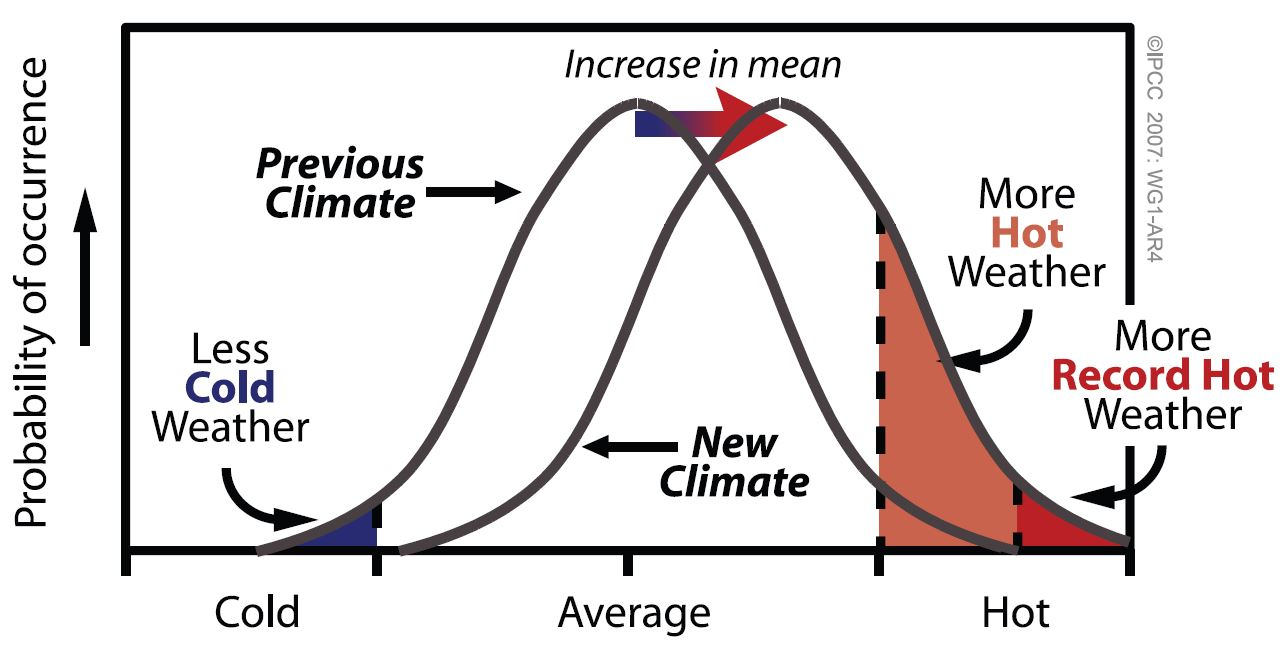
\includegraphics{figs/Fig1.1.jpg}
\caption{\label{fig:fig-1-1}Schematic showing the increase in frequency of extreme
temperatures (shaded light pink) and the magnitude of extreme
temperatures (shaded dark pink), in response to increasing mean
temperature for a normal distribution of temperatures. `extreme' refers
to events that would have been anomalous under the previous probability
distribution. Figure taken directly from \citet{ipcc_climate2007}.}
\end{figure}

\subsubsection{Range shifts due to climate
change}\label{range-shifts-due-to-climate-change}

Species may track optimal climatic conditions by shifting their range.
This commonly occurs through net population extinctions at the trailing
edge, or net population colonisations at the leading edge
\citep{parmesan_poleward1999}. Dispersal by individuals may also occur
in highly mobile species. Since the predominant effect of climate change
is increasing temperature, many species track temperature by moving to
higher latitudes --- as exemplified in the Arctic, where organisms such
as shrubs and red foxes have expanded polewards
\citep{hersteinsson_interspecific1992, sturm_climate2001}. Others move
to higher altitudes; both latitudinal and altitudinal shifts have been
seen in birds and butterflies of temperate regions
\citep{hill_responses2002, parmesan_poleward1999, thomas_birds1999}.

Until recently, there were very few studies of range shifts due to
climate change in tropical species, with some suggesting that the
response should be less extreme given the slower rates of warming in the
tropics \citep{freeman_rapid2014, stocker_climate2013}. It is now
apparent that tropical species do shift their ranges to track climate,
particularly to higher elevations
\citep{chen_elevation2009, pounds_biological1999} owing to shallow
temperature gradients across latitudes \citep{colwell_global2008}. In
fact, tropical species track climate more closely than temperate species
\citep{freeman_rapid2014}. This effect could be due to: (1) greater
thermal specialisation as a result of long-term thermal stability in the
tropics \citep{freeman_rapid2014}; (2) slower velocity of climate change
up mountains \citep{loarie_velocity2009} meaning it is easier for
species to keep pace; or (3) fewer barriers to dispersal in the tropics,
since tropical biomes have thus far retained a greater proportion of
natural habitat than temperate regions. In any case, even tropical
species do not track climate precisely \citep{chen_elevation2009}.

\subsubsection{In situ adaptation to climate
change}\label{in-situ-adaptation-to-climate-change}

In situ adaptation encompasses biochemical buffering, gene expression,
phenotypic plasticity, behaviour and genetic adaptation
\citep{peck_organisms2011}. Adaptation is complex and largely
unpredictable; hence it is rarely accounted for in models used to
predict range shifts \citep{peck_organisms2011}. This may be one of the
reasons that species do not move as quickly as predicted.

Modifications in species' phenology represent the vast majority of
documented adaptations to climate change in situ. Many of these examples
come from temperate regions of the Northern hemisphere, where
seasonality is the overarching determinant of species' phenology, and is
itself dramatically altered by climate change
\citep{bradshaw_evolutionary2006}. Specifically, spring has advanced and
the growing season has lengthened. Organism responses include earlier
breeding in animals such as birds and butterflies, earlier arrival of
migratory birds, and earlier flowering in plants
\citep{walther_ecological2002}.

Responses such as physiological plasticity or genetic adaptation feature
much less in the literature on in situ adaptation to climate change.
This may signify a real scarcity of such changes in nature. The
evolution of new forms that enable persistence in the same geographic
range under a changing climate requires a species to become tolerant of
a climatic regime to which it was previously intolerant, which seems
unlikely \citep{parmesan_ecological2006}. One could argue that selective
pressures to evolve increased thermal tolerance would have been
insufficient prior to present-day climate change. However, major
evolution at the species level is not evident in the fossil record
during the Pleistocene glaciation event, even though this comprised
climate change of 5-10 times the magnitude of 20th Century warming
\citep{parmesan_ecological2006}.

While evidence for evolutionary responses to climate change is limited,
this is not to say that evolution has no role to play. Where examples of
such responses do exist, they underlie aforementioned ecological changes
in phenology or dispersal \citep{parmesan_ecological2006}. For example,
Dutch great tits that display greater plasticity in their timing of
reproduction are better able to match egg-laying to food availability --
the peak of which has advanced as a result of climate change -- and thus
achieve greater fitness \citep{nussey_selection2005}. There are also
practical explanations for the lack of documented evolutionary
responses, since these adaptations are less intuitive and harder to
document than ecological responses \citep{oconnor_toward2012}.

The literature discussed above fails to mention one additional and very
significant tool that animals can employ to adapt to climate change --
behaviour. All organisms ordinarily experience a range of temperatures,
and so possess thermoregulatory behaviours that can also be deployed to
mitigate the impacts of climate change. Chamois, for example, move to
higher altitudes and reduce activity when temperature increases
\citep{mason_predicting2014}.

Habitats present a considerable degree of variation in microclimates,
because of variation in microhabitat features
\citep{scheffers_microhabitats2014}, slope and aspect
\citep{suggitt_habitat2011}. Behavioural plasticity allows animals to
move into these microclimates \citep{scheffers_microhabitats2014} and so
track their optimal climate on a local scale. These so-called
``microrefugia'' are utilised by a variety of taxa around the world. In
boreal forests of Finland, moose seek out the cooler microclimates of
forests with higher and denser canopies, in response to high daytime
temperatures \citep{melin_moose2014}. Similarly, in the tropics, possums
choose the coolest tree hollows in which to den
\citep{isaac_microclimate2008}, and herpetofauna of Singapore occupy
microrefugia that not only largely avoid their critical thermal maxima
(CT\textsubscript{max}) -- which is often exceeded in the wider
macroclimate -- but their microrefugia also heat less quickly than the
macroclimate \citep{scheffers_microhabitats2014}.

\section{Influence of land-use
change}\label{influence-of-land-use-change}

The most well-known interaction between climate change and land-use
change is probably that the latter can cause the former, on a global
scale, through the release of GHGs \citep{stocker_climate2013}.
Deforestation marginally reduces the net radiative forcing that leads to
global climate warming through decreases in surface albedo
\citep{stocker_climate2013}. Climate change could also cause land-use
change, such as through shifting the areas which are most climatically
suited for agriculture \citep{opdam_climate2004}.

In this review, however, I have focused on how organisms can adaptively
respond to change. The question then becomes: how does land-use change
influence an organism's capacity to respond to climate change? On a
regional scale under wholesale conversion, the answer is relatively
well-discussed. Namely, regional habitat loss creates barriers to
climate-driven range shifts \citep{thomas_protected2012}. Recall that in
response to climate change that has already happened, organisms have not
moved as quickly as expected \citep{chen_elevation2009}, and barriers to
dispersal may contribute to this.

In situ adaptation may allow organisms to persist in habitats from which
they are unable to move, or it may remove the need to move altogether;
in either case, the influence of land-use change on in situ adaptation
to climate change has not been elucidated. Given that many barriers to
dispersal have already been introduced, and this will likely continue
into the future, it is vital to facilitate adaptation to future climate
change within the areas that species already occupy.

Most obviously, wholesale conversion of natural or semi-natural habitat
appears to increase local daytime mean temperature
\citep[e.g.][]{wickham_comparison2012}. Largely, this is caused by an
increase in daily maximum temperature as a result of decreased
interception by overhead vegetation of direct solar radiation
\citep{xu_scale-dependent2004}. The effect is reversed at night when
outgoing long-wave radiation is lost because of reduced interception by
vegetation \citep{xu_scale-dependent2004}. An increase in mean
temperature may exceed an organism's preferred body temperature, and so
potentially lead to sublethal effects \citep{du_plessis_costs2012}, but
increasing maximum temperature generally poses the greater threat to
organisms. Organisms can often acclimate to moderate increases in
average temperatures \citep{peck_animal2009}, but if their critical
thermal maximum is exceeded -- even for a very short amount of time --
this will cause death. Thus, species remaining in habitat after it has
been converted are already likely to be under some amount of thermal
stress, and future climate change may push temperatures beyond the range
that they can tolerate through physiological plasticity.

Any increase in ambient temperature will ultimately increase the
temperature of microclimates, and so potentially decrease their efficacy
as thermal microrefugia for thermally stressed individuals. The extent
to which microclimate utility is compromised depends upon the rate at
which they warm alongside macroclimate warming. There is evidence from
the tropics that this relationship is non-uniform, with microhabitat
temperatures increasing only 0.11--0.66°C for every 1°C in the
macroenvironment \citep{scheffers_microhabitats2014}. Asymmetry in
warming rates will be influenced by factors that act to create the
microclimate, such as the microhabitat
\citep{scheffers_microhabitats2014}, slope, aspect or elevation
\citep{suggitt_habitat2011}. It is possible that microclimates could be
entirely removed as a consequence of microhabitat removal
\citep[e.g.~loss of some bird's nest fern species upon conversion of
forest to oil palm plantation;][]{fayle_effect2009} or extreme
macroclimate warming \citep{caillon_warming2014}.

Wholesale conversion is very likely to impede the ability of persisting
organisms to adapt to future climate change, but then few of the
original species do persist through conversion
\citep[e.g.][]{gibson_primary2011, katovai_understory2012, murphy_meta-analysis2014}
and --- at least in the tropics --- habitat degradation is far more
pervasive. In particular, some 20\% of the humid tropical biome
experienced selective logging from 2000-2005
\citep{asner_contemporary2009}, whilst deforestation affected only 1.4\%
in the same period \citep{hansen_humid2008}. Although the habitat type
broadly remains as `forest', selective logging can be extremely
disruptive. Indeed the term `selective' is somewhat of a misnomer,
meaning that particular species and stems (usually above a minimum trunk
diameter) are targeted \citep{edwards_maintaining2014}. These targets
are typically the largest, oldest trees, the removal of which reduces
canopy height and canopy density
\citep{kumar_effects2005, okuda_effect2003}, and also fragments the
forest canopy and opens up large gaps \citep{edwards_maintaining2014}
that are often invaded by non-tree species, such as climbers and bamboo.
Commercial selective logging also causes collateral damage, particularly
where trees are connected by climbers \citep{schnitzer_recruitment2004},
as well as requiring roads and skid trails that bring further challenges
for wildlife \citep{brodie_correlation2014, laurance_global2014}, and
heavy machinery that result in soil compaction
\citep{putz_reduced-impact2008}.

Since selective logging reduces canopy cover, just as deforestation
does, so it is likely that the thermal regimes of degraded forest will
be similarly altered. Moreover, there is already some indication that
previously identified tropical microrefugia \citep[in this case, leaf
litter and soil;][]{scheffers_microhabitats2014}, are reduced by logging
\citep{saner_reduced2009}. Conversely, ground vegetation --- another
microrefugium \citep{scheffers_microhabitats2014} --- may be favoured by
the release of pioneer species upon the creation of treefall gaps.

The impact of habitat degradation on species' ability to persist under
climate change is likely to be less profound than under wholesale
conversion, simply because the amount of habitat change is less.
However, a greater proportion of species found in undisturbed habitat
remain in degraded habitat than in converted habitat
\citep{edwards_degraded2011}, and it is these species that are of
primary conservation concern. Furthermore, degraded forests now
represent a significant proportion of the humid tropical biome, and are
therefore home to a significant proportion of all tropical forest
species on Earth. The potential for these species to track climate
change through dispersal is limited -- there are barriers, such as
hostile land-use types, as well as a shallow latitudinal temperature
gradient \citep{colwell_global2008} and a potential lack of connected,
higher elevation habitat \citep{scriven_protected2015}. Many tropical
species will need to adapt to climate change within degraded forest, if
they are to persist into the future. Therefore, although we do not yet
fully understand the impact of any land-use change on the ability of
tropical species to adapt in situ to climate change, I argue that we
should first explore the impacts of habitat degradation, as a priority.

\section{Thesis aims and rationale}\label{thesis-aims-and-rationale}

\subsubsection{Definitions}\label{definitions}

`Microhabitats' are fine-scale (mm to cm) features within a habitat,
including leaf litter, deadwood, tree holes and epiphytes within
rainforest habitats. Each of these features will have its own
`microclimate' which may be different from the macroclimate that acts at
the level of the whole habitat (m to ha). When microhabitat features
offer a more desirable microclimate than the macroclimate, the features
can be referred to as `thermal microrefugia' (`microrefugia'
henceforth).

\subsubsection{Chapter 2 -- A pantropical analysis of the impacts of
forest degradation and conversion on local
temperature}\label{chapter-2-a-pantropical-analysis-of-the-impacts-of-forest-degradation-and-conversion-on-local-temperature}

SUMMARY

\subsubsection{Chapter 3 -- A framework for quantifying fine-scale
thermal heterogeneity in the
field}\label{chapter-3-a-framework-for-quantifying-fine-scale-thermal-heterogeneity-in-the-field}

SUMMARY

\subsubsection{Chapter 4 -- Tropical forests are thermally buffered
despite intensive selective
logging}\label{chapter-4-tropical-forests-are-thermally-buffered-despite-intensive-selective-logging}

SUMMARY

\subsubsection{Chapter 5 -- The impact of recent forest cover change on
climate connectivity in the
tropics}\label{chapter-5-the-impact-of-recent-forest-cover-change-on-climate-connectivity-in-the-tropics}

SUMMARY

\section{References}\label{references}

\chapter{A pantropical analysis of the impacts of forest degradation and
conversion on local
temperature}\label{a-pantropical-analysis-of-the-impacts-of-forest-degradation-and-conversion-on-local-temperature}

\section{Abstract}\label{abstract}

Temperature is a core component of a species' fundamental niche. At the
fine scale over which most organisms experience climate (mm to ha),
temperature depends upon the amount of radiation reaching the Earth's
surface, which is principally governed by vegetation. Tropical regions
have undergone widespread and extreme changes to vegetation,
particularly through the degradation and conversion of rainforests.
Since most terrestrial biodiversity is in the tropics, and many of these
species possess narrow thermal limits, it is important to identify local
thermal impacts of rainforest degradation and conversion. We collected
pantropical, site-level (\textless{} 1 ha) temperature data from the
literature to quantify impacts of land-use change on local temperatures,
and to examine whether this relationship differed above-ground relative
to below-ground and between wet and dry seasons. We found that local
temperature in our sample sites was higher than primary forest in all
human-impacted land-use types (N = 113,894 day-time temperature
measurements from 25 studies). Warming was pronounced following
conversion of forest to agricultural land (minimum +1.6°C, maximum
+13.6°C), but minimal and non-significant when compared to forest
degradation (e.g.~by selective logging; minimum +1°C, maximum +1.1°C).
The effect was buffered below-ground (minimum buffering 0°C, maximum
buffering 11.4°C), whereas seasonality had minimal impact (maximum
buffering 1.9°C). We conclude that forest-dependent species that persist
following conversion of rainforest have experienced substantial local
warming. Deforestation pushes these species closer to their thermal
limits, making it more likely that compounding effects of future
perturbations, such as severe droughts and global warming, will exceed
species' tolerances. By contrast, degraded forests and below-ground
habitats may provide important refugia for thermally-restricted species
in landscapes dominated by agricultural land.

\bibliography{Ch2,Ch1}


\end{document}
